\documentclass[compress]{beamer}
% By  using hyperref={pdfpagelabels=false} you get rid off:
% Package hyperref Warning: Option `pdfpagelabels' is turned off
% (hyperref)                because \thepage is undefined. 
% Hyperref stopped early 
%

\usepackage{lmodern}
\usepackage{graphicx}
%\usepackage{caption}
\usepackage{subcaption}

\usepackage{verbatim}
% Using lmondern and you get rid off this:
% LaTeX Font Warning: Font shape `OT1/cmss/m/n' in size <4> not available
% (Font)              size <5> substituted on input line 22.
% LaTeX Font Warning: Size substitutions with differences
% (Font)              up to 1.0pt have occurred.
%

% If \titel{$B!D(B} \author{$B!D(B} come after \begin{document} 
% you get the following warnig:
% Package hyperref Warning: Option `pdfauthor' has already been used,
% (hyperref) ... 
% So it is here before \begin{document}

\providecommand\thispdfpagelabel[1]{}

%\title{QSAR and Meta-Learning: can we improve Drug Design \& Discovery?}   
%\author{Noureddin SadawiBrunel University - London} 
%\date{\today} 

\title[Meta-QSAR EPSRC Project Meeting 19/20 Feb 2015] % (optional, only for long titles)
{Meta-QSAR EPSRC Project Meeting 19/20 Feb 2015}
%\subtitle{Can we improve Drug Design \& Discovery?}
\author[Brunel University Team] % (optional, for multiple authors)
{Brunel University Team}
\institute[Brunel University - London] % (optional)
{
  Dept of Computer Science\\
  Brunel University 
}
\date[\today] % (optional)
%{Meta-QSAR Meeting}
%{How Scientific Collaboration can boost our Research\\At Bournemouth University}
%\subject{Computer Science}

%\usepackage{beamerthemesplit} % new 
% Alternatively, you can also use the usetheme Warsaw
\usetheme{Dresden}
\setbeamertemplate{headline}{}


\begin{document}

\begin{frame}
\titlepage
\end{frame} 

\begin{frame}
\frametitle{Table of contents}
\tableofcontents
\end{frame}
 
\begin{comment} 
\section{Research Team} 
\begin{frame}
\frametitle{Teams Involved in this Project } 
\begin{itemize}
\item University of Manchester
\begin{itemize}
\item Prof Ross D. King
\item Dr Ivan Olier
\end{itemize}
\item Brunel University
\begin{itemize}
\item Dr Larisa Soldatova
\item Dr Noureddin Sadawi
\end{itemize}
\item University of Dundee
\begin{itemize}
\item Prof Andrew Hopkins
\item Dr Jeremy Besnard
\item Dr Richard Bickerton
\item Dr Willem van Hoorn
\end{itemize}

%\item The use of descriptors of physical properties allow for the application of mathematical models to analyze and predict drug activity
%\item These properties are evaluated using molecular descriptors

\end{itemize}
\end{frame}


\section{QSAR} 
\begin{frame}
\frametitle{Quantitative Structure-Activity Relationship (QSAR) 1/2} 
\begin{itemize}
\item Drugs are small molecules
\item Drug Targets are large molecules (e.g. proteins) 
\item The biological activity of drugs is (largely) dictated by their properties
%\item The physical properties of drugs, in part, dictate their biological activity
%\item Mapping of structure of drugs into assay activity (regression)
%\item How do we represent small molecules? FP's, LogP

\item The use of descriptors of physical properties allows for the application of mathematical models to analyze and predict drug activity

%\item These properties are evaluated using molecular descriptors

\end{itemize}
\end{frame}

\begin{frame}
\frametitle{Quantitative Structure-Activity Relationship (QSAR) 2/2} 
\begin{itemize}
\item Descriptors $\rightarrow$ Mathematical Models $\rightarrow$ Analysis and Prediction of Drug Activity
\item QSAR is used to analyze experimental data and build numerical models for prediction and interpretation purposes
%\item Maps structure of drugs to assay activity (regression)

\item Uses a set of molecules whose activity in a particular experiment is known
\item Given such set, a QSAR model correlates these activities with properties of molecules in the set

\item Used to guide the synthesis of more potent drugs

\end{itemize}
\end{frame}


%\begin{frame}
%\frametitle{Quantitative Structure-Activity Relationship (QSAR) 3/4} 
%Here we have tsar Fig \\
%Download it from PC

%\begin{figure}[h!]
  %\caption{A picture of a gull.}
 % \centering
   % 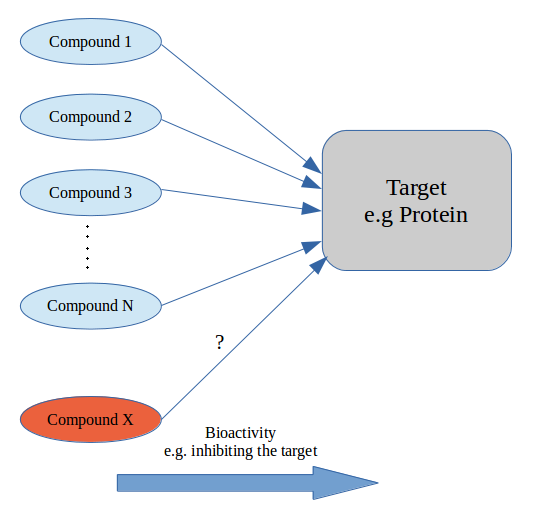
\includegraphics[width=0.5\textwidth]{qsar}
%\end{figure}

%\end{frame}

%\begin{frame}
%\frametitle{Quantitative Structure-Activity Relationship (QSAR) 4/4} 
%\begin{itemize}
%\item FPs and Descriptors 23:13

%\end{itemize}
%\end{frame}


\section{Meta-learning}
\begin{frame}
\frametitle{Meta-learning and Machine Learning (ML)} 
\begin{itemize}%[<+->]
\item The possibility of using ML to address some of the problems ML researchers face in ML %\pause 
\item \emph{Metadata:} the type of data that may be viewed as being generated through the application of machine learning
\item \emph{Metalearning:} the use of machine learning techniques to build models from metadata %\pause 
\item An important problem is \emph{algorithm selection} %\pause 

%\item Open QSAR is also a platform that facilitates the meta analysis of QSAR model libraries carried out by combining the results of all modelling studies and comparing the performance of components such as data transformation, descriptor calculation, feature selection and modelling methods as well as temporal changes through model updating. 

\end{itemize}

\end{frame}

\section{Meta-QSAR}
\begin{frame}
\frametitle{Meta-learning and QSAR} 
\begin{itemize}%[<+->]
\item There is no single best way of learning QSAR (nearly all algorithms have been used in QSAR)
\item There exists little guidance on which QSAR approach to use for a certain problem
\item We are trying to learn how to better apply existing QSAR methods
\item We will use machine learning to learn about QSAR learning
\end{itemize}

\end{frame}

\section{The Data}
\begin{frame}
\frametitle{The ChEMBL Database} 
\begin{itemize}%[<+->]
\item A freely available resource for drug discovery data (searchable and downloadable)
\item New data released regularly
\item Medicinal Chemistry literature is analysed for drug discovery data
\item Compounds interacting with Specific Targets can be identified easily
\item Searching:
  \begin{itemize}%[<+->]
   \item Search for protein names/synonyms (text search)
   \item Search by compound name (e.g. drug name or smiles)
  \end{itemize}
\end{itemize}

\end{frame}
\end{comment} 

\section{Receiving Dataset from Dundee Team}
\begin{frame}
\frametitle{Receiving Dataset from Dundee Team} 
\begin{itemize}%[<+->]
 \item The Dundee team (specifically Jeremy) sent us the datasets
 \item It contains activity data for compounds per targets (MEDIAN\_PXC50 and ACTIVITY\_FLAG)
 \item A threshold was used to obtain ACTIVITY\_FLAG from MEDIAN\_PXC50
 \item The Manchester and Brunel teams decided to use MEDIAN\_PXC50 (after advice from Ross)
\end{itemize}
\end{frame}


\section{Evaluation Metrics}
\begin{frame}
\frametitle{Classification or Regression} 
\begin{itemize}%[<+->]
\item Before Ross's advice we (at Brunel) worked on metrics for Regression and Classification tasks
\item We Studied Ontologies such as Expose and DMOP
\item Much more metrics for Classification
\item Studied WEKA in Depth
%\item List of metrics
\end{itemize}
\end{frame}


\begin{frame}
\frametitle{Metrics in Weka} 
\begin{figure}[h!]
  %\caption{A picture of a gull.}
  \centering
    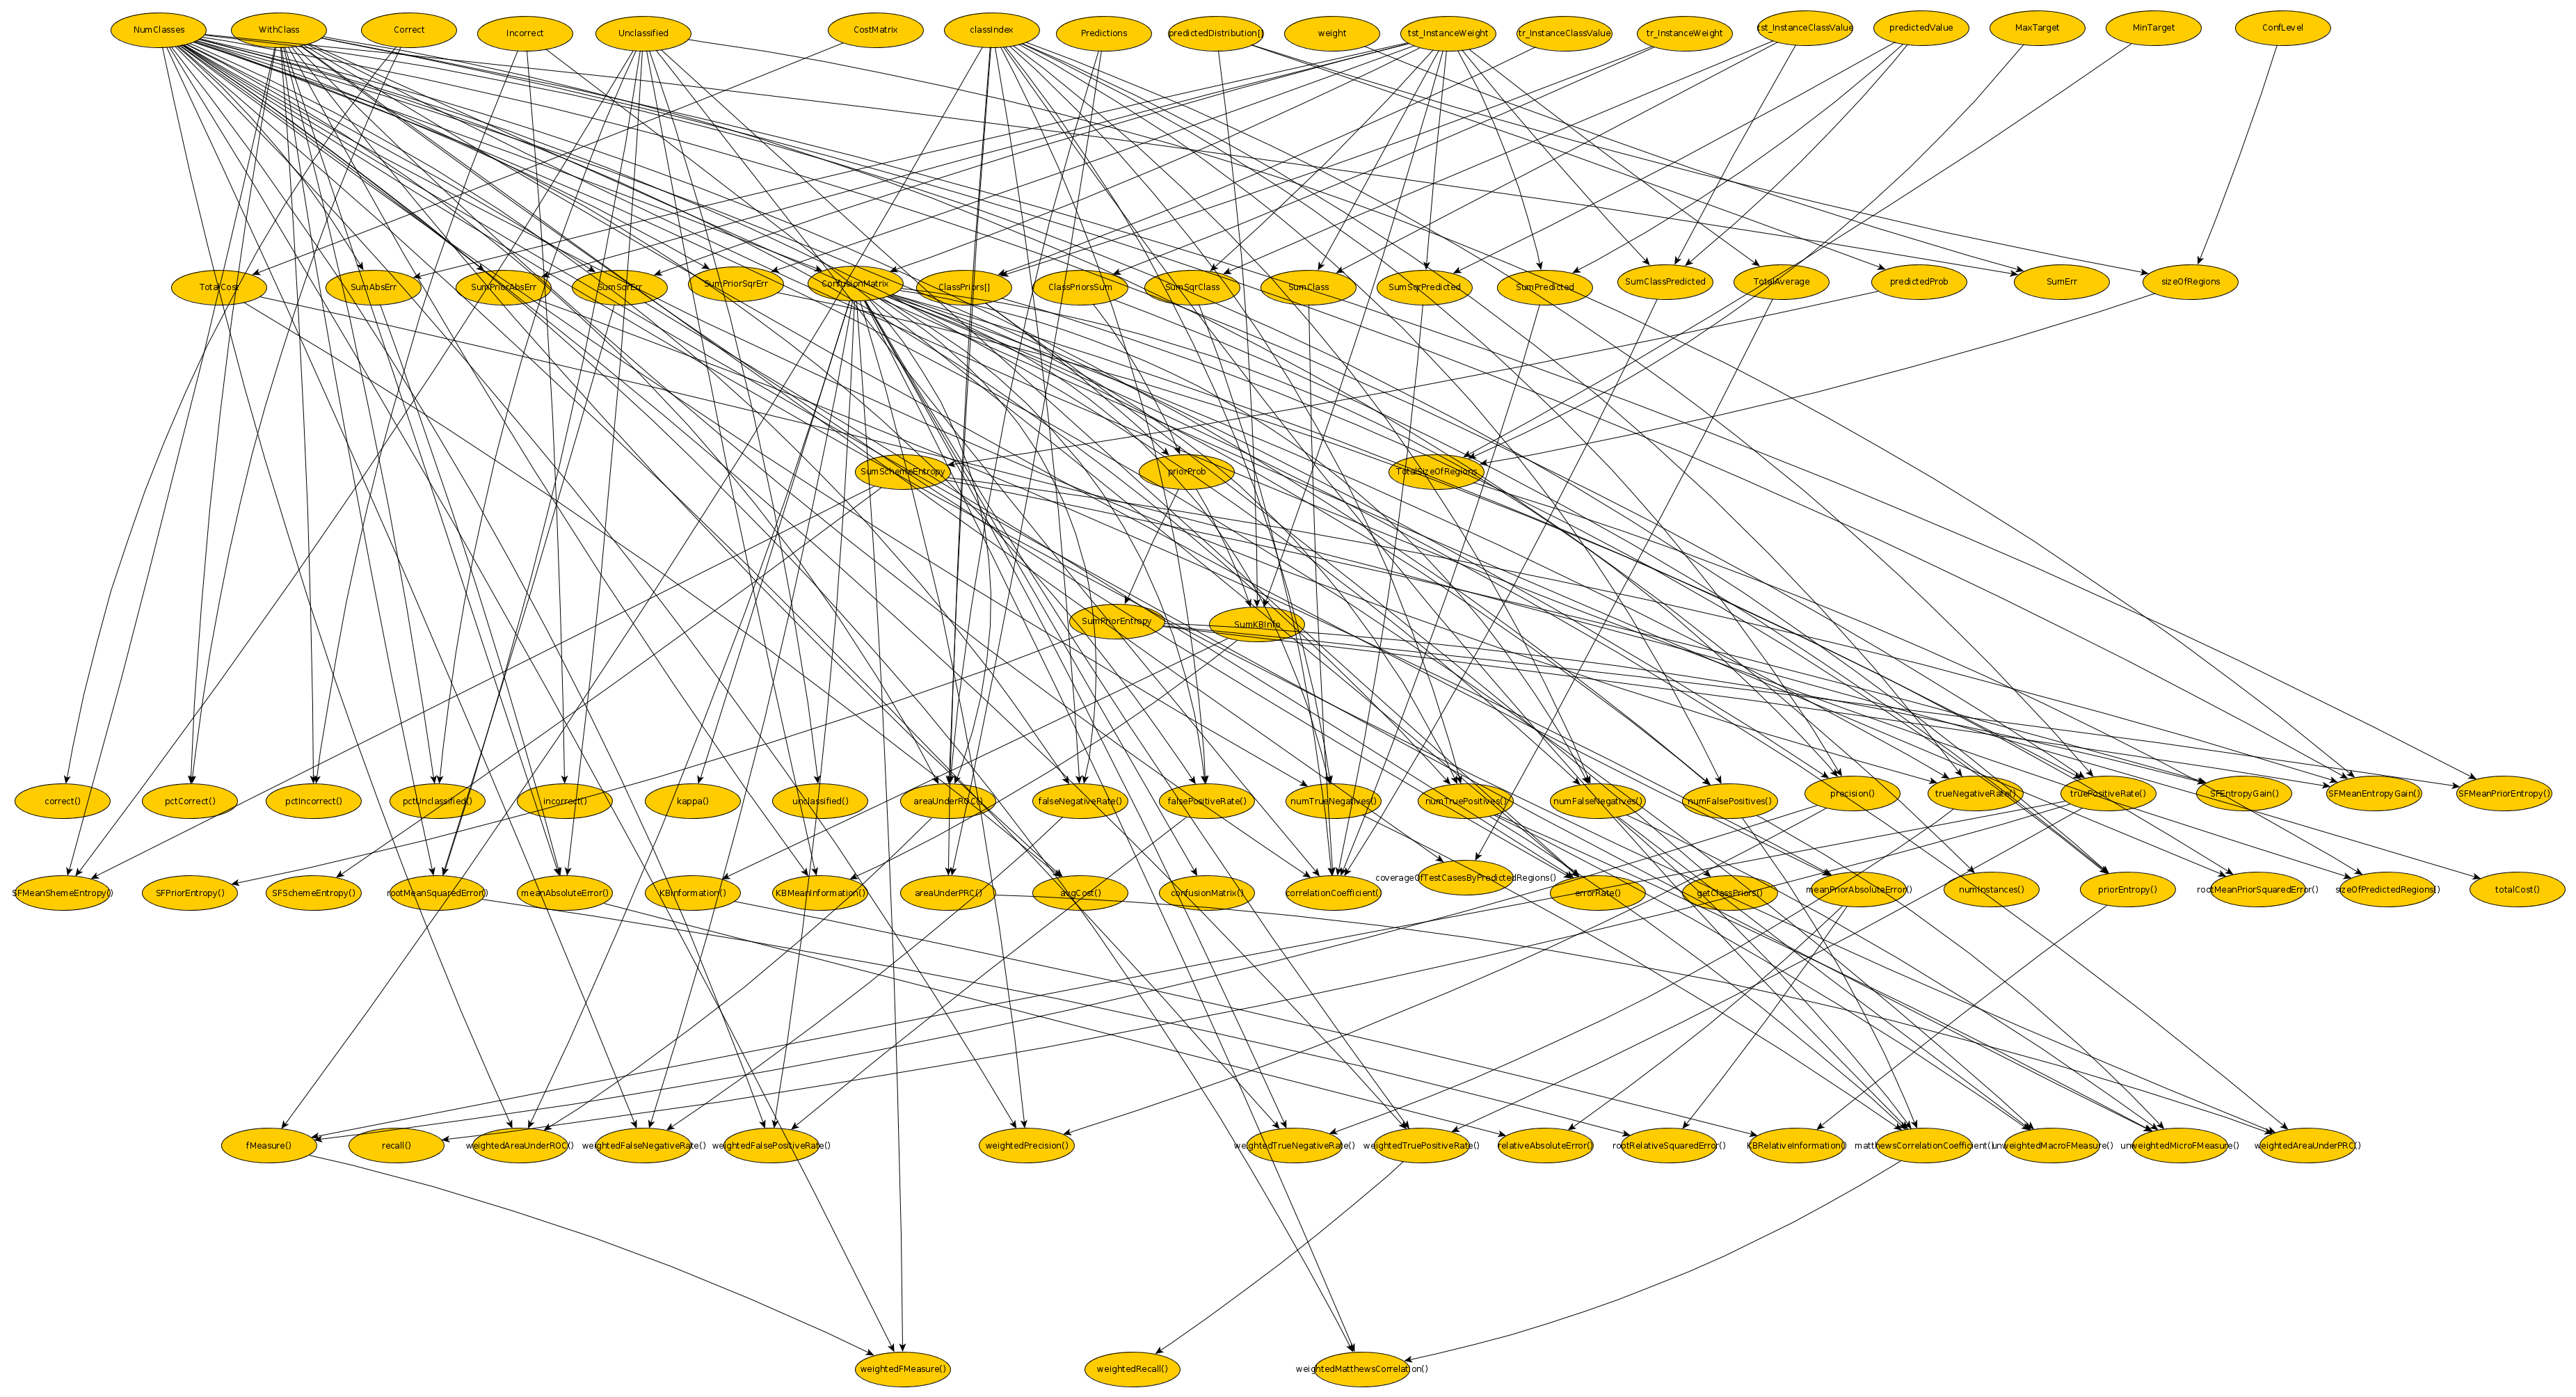
\includegraphics[width=1.05\textwidth]{weka-metrics}
\end{figure}
\end{frame}


\begin{frame}
\frametitle{Metrics for Regression} 
\begin{itemize}%[<+->]
\item List of metrics:
\begin{itemize}%[<+->]
\item Root mean square error
\item Mean of absolute errors
\item Median of absolute errors
\item Median of squared errors
\item Mean of squared errors
\item Sum of absolute errors
\item Sum of squared errors
\end{itemize}
\end{itemize}
\end{frame}



\section{Database Design}
\begin{frame}
\frametitle{Database Design} 
\begin{itemize}%[<+->]
 \item Worked closely with the Manchester team to design an initial database
 \item Iterative process
 \item We kept compatibility with OpenML in mind
 \item Currently Ivan is in control of it (and many thanks to him)
\end{itemize}
\begin{figure}[h!]
  %\caption{A picture of a gull.}
  \centering
    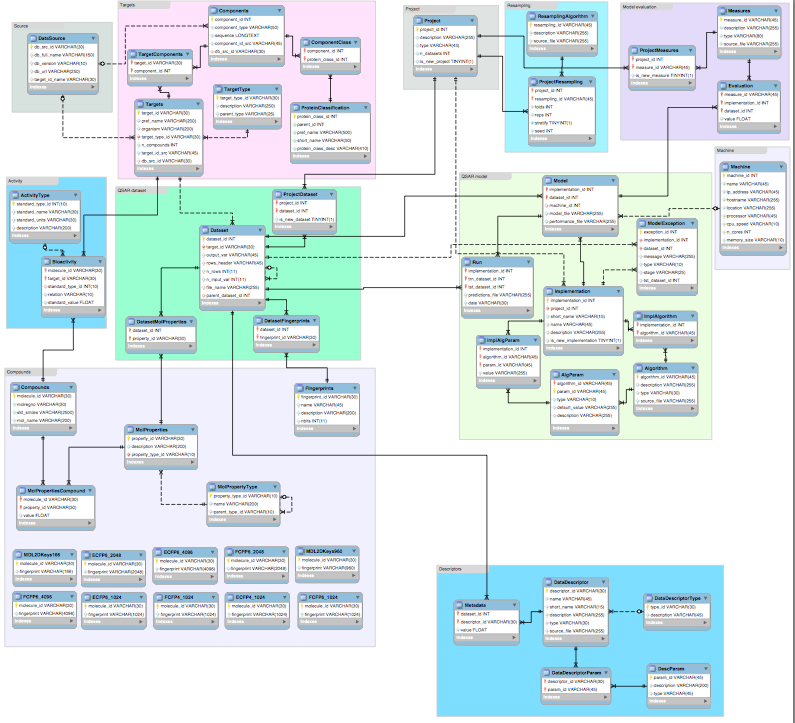
\includegraphics[width=0.5\textwidth]{ourdb}
\end{figure}
\end{frame}


\section{Metadata \& Classification of Targets}
\begin{frame}
\frametitle{Metadata} 
\begin{itemize}%[<+->]
%\item About small molecules (drugs)
%\item Meta-learning requires data about base level learning problems or tasks, i.e., training metadata
\item About datasets (metadata)
\item About drug targets (metadata)
\end{itemize}



\end{frame}

\begin{frame}
\frametitle{Data on Datasets} 
\begin{itemize}%[<+->]
  \item We compute several general dataset meta-features such as:
  \begin{itemize}
  \item mutual information
  \item equivalent number of attributes
  \item noise to signal ratio
  \end{itemize}
  \item We also compute some domain specific ones (diversity indices) such as:
  \begin{itemize}
  \item generic diversity index
  \item explicit diversity index
  \end{itemize}
\end{itemize}
\end{frame}

%\section{Classification of Targets}
\begin{frame}
\frametitle{Classification of Targets} 
\begin{itemize}%[<+->]
  \item Exchanged emails with Richard regarding Classification of Targets
  \item Decided to exclude targets with multiple components (protein families)
  \item Knowing protein family in advance should be advantageous
  \item Analysis of groups of drug targets
  \item Possibly group targets in a more useful/meaningful way  
  \item Currently the Manchester team is dealing with this
\end{itemize}
\end{frame}
 



\section{Database Backup}
\begin{frame}
\frametitle{Database Backup} 
\begin{itemize}%[<+->]
 \item In the unlikely event of data loss/damage
 \item We perform nightly back up of databases to Brunel
 \item Currently:
    \begin{itemize}%[<+->]
       \item qsars\_db
       \item metaqsar\_db
    \end{itemize}
\end{itemize}
\end{frame}



\section{OpenML}

\begin{frame}
\frametitle{Special Section on OpenML} 
\begin{itemize}%[<+->]
 %\item We would like to have a special section on OpenML
 \item Initially we would like the data to be private (e.g. accessible by certain people)
 \item We would like to be able to make the data public at the appropriate time
 \item Maybe have a special QSAR section on OpenML
\end{itemize}
\end{frame}


\begin{frame}
\frametitle{Uploading Datasets and Results to OpenML} 
\begin{itemize}%[<+->]
 \item Two options (either openml repeats experiments or we provide details of results)
 \item We will upload our datasets and results (telling openml all it needs to carry out comparisons)
 \item We can upload in more than one way (e.g. R, java, PHP)
 \item PHP Code Demonstration
\end{itemize}
\end{frame}

\begin{frame}
\frametitle{Connect to OpenML via API} 
%Here we have tsar Fig \\
%Download it from PC

\begin{figure}[h!]
  %\caption{A picture of a gull.}
  \centering
    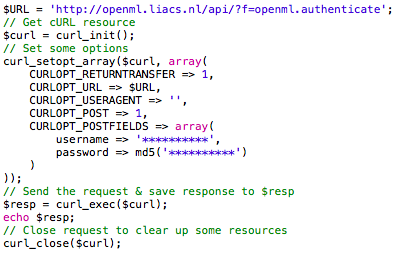
\includegraphics[width=0.85\textwidth]{openml-connect}
\end{figure}

\end{frame}

\begin{frame}
\frametitle{Upload Dataset to OpenML via API} 
%Here we have tsar Fig \\
%Download it from PC

\begin{figure}[h!]
  %\caption{A picture of a gull.}
  \centering
    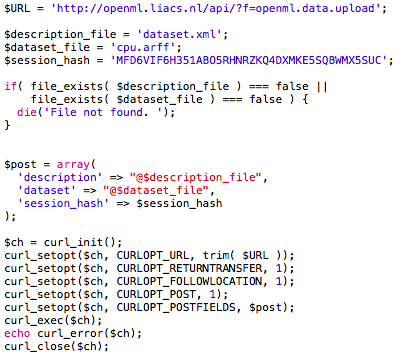
\includegraphics[width=0.75\textwidth]{openml-ds}
\end{figure}

\end{frame}

\begin{frame}
\frametitle{Upload Run to OpenML via API} 
%Here we have tsar Fig \\
%Download it from PC

\begin{figure}[h!]
  %\caption{A picture of a gull.}
  \centering
    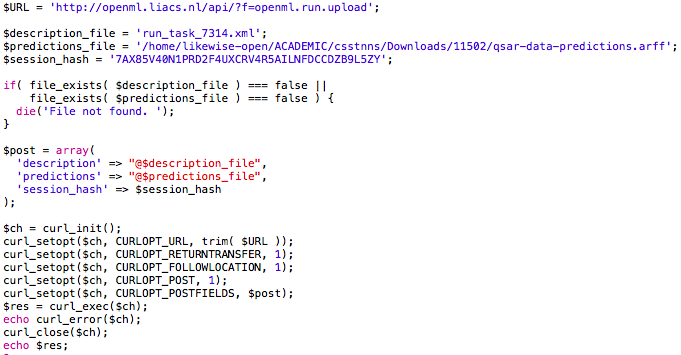
\includegraphics[width=1.10\textwidth]{openml-run}
\end{figure}

\end{frame}


\section{Another Project Underway: Transfer Learning}
\begin{frame}
\frametitle{Transfer Learning} 
\begin{itemize}%[<+->]
 \item Transfer learning deals with the ability of a system to recognize and apply knowledge and skills learned in previous tasks to novel tasks
 \item It aims to extract the knowledge from one or more source tasks (data with known classes) and applies the knowledge to a target task (data with unknown classes)
 \item Traditional machine learning techniques try to learn each task from scratch, while transfer learning techniques try to transfer the knowledge from some previous tasks to a target task when the latter has fewer high-quality training data
\end{itemize}
\end{frame}

\begin{frame}
\frametitle{Inductive Transfer Learning} 
\begin{itemize}%[<+->]
 \item \textbf{Instance-transfer:} To re-weight some labeled data in a source domain for use in the target domain %(I think this is suitable for our purposes - Noureddin)
 \item \textbf{Feature-representation-transfer:} Find a good feature representation that reduces difference between a source and a target domain or minimizes error of models
 \item \textbf{Model-transfer:} Discover shared parameters or priors of models between a source domain and a target domain
 \item \textbf{Relational-knowledge-transfer:} Build mapping of relational knowledge between a source domain and a target domain
 \end{itemize}
\end{frame}

\begin{frame}
\frametitle{Instance-Transfer Learning} 
\begin{itemize}%[<+->]
 \item The instance-transfer approach to the inductive transfer learning setting is intuitively appealing
 \item \textbf{Assumption:} the source domain and target domain data use exactly the same features and labels
 \item \textbf{Motivation:} Although the source domain data can not be reused directly, there are some parts of the data that can still be reused by re-weighting
 \item \textbf{Main Idea:} Discriminatively adjust weights of data in the source domain for use in the target domain 
 \end{itemize}
\end{frame}

\begin{frame}
\frametitle{Targets and their Sequences} 
\begin{itemize}%[<+->]
 \item Currently we are working on data for three organisms:
 \begin{itemize}%[<+->]
   \item Homo Sapiens
   \item Plasmodium Falciparum (parasite)
   \item Plasmodium Vivax (parasite)
 \end{itemize}
  
  \item The data is from assays carried out by Eve Robot Scientist

 \item We use sequences to check how similar these targets are (the UniProt database)
 \end{itemize}
\end{frame}

\begin{frame}
\frametitle{UniProt} 
\begin{itemize}%[<+->]
 \item UniProt (www.uniprot.org) is a manually curated database which focuses on protein sequences
 \item Curators at UniProt pay much attention to the amount and quality of information about proteins
 \item Each protein has a UniProt entry
 \item Other major databases (e.g. NCBI, ChEMBL, DrugBank) link to it
 
 \end{itemize}
\end{frame}


\begin{frame}
\frametitle{Retrieving a UniProt Protein Sequence} 
\begin{itemize}%[<+->]
 \item Searching for the full protein name + the organism name, i.e. dihydrofolate reductase organism: "homo sapiens"
 \item This will return several entries
 \item Some entries have different colours and they are \textbf{reviewed}
 
 \end{itemize}
\end{frame}


\begin{frame}
\frametitle{Our Idea} 
\begin{itemize}%[<+->]
 \item What we would like to test is whether we can transfer what we learn about one parasite to another parasite
 \item We can measure the distance (or similarity) between parasites using their sequences 
 \item Our current assumption is that the more different (or more far apart) the parasites the more difficult (or less accurate) transfer learning becomes
 
%What we transfer is the difference in activity between human and parasites. In more detail, we transfer the difference in activity between a human (where drug is inactive) and one parasite (where drug is active) to another parasite (about which we have little data)
 \end{itemize}
\end{frame}

\begin{comment}
\begin{frame}
\frametitle{Comparing Two Sequences Graphically} 
\begin{itemize}%[<+->]
 \item here have the four figures for comparison
 
%What we transfer is the difference in activity between human and parasites. In more detail, we transfer the difference in activity between a human (where drug is inactive) and one parasite (where drug is active) to another parasite (about which we have little data)
 \end{itemize}
\end{frame}
\end{comment}

\begin{frame}
\frametitle{Comparing Two Sequences Graphically} 
\begin{figure}[h!]
  %\caption{A picture of a gull.}
  \centering
   
   \begin{subfigure}[b]{0.35\textwidth}
    \centering
    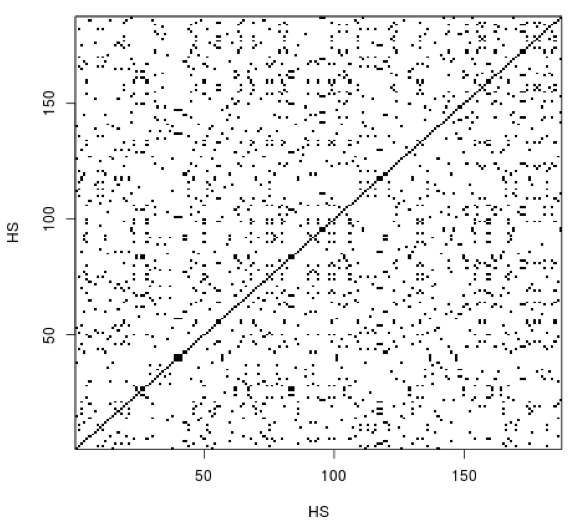
\includegraphics[width=1.0\textwidth]{hs-hs}
   \end{subfigure}
   %\hfill
    \begin{subfigure}[b]{0.35\textwidth}
    \centering
    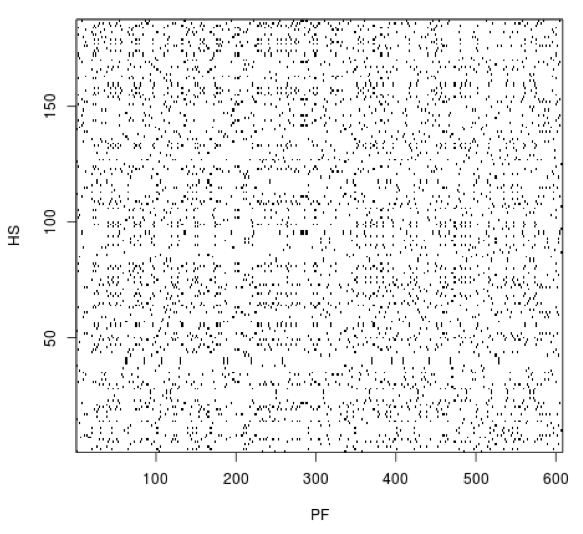
\includegraphics[width=1.0\textwidth]{hs-pf}
   \end{subfigure}
   
   \begin{subfigure}[b]{0.35\textwidth}
    \centering
    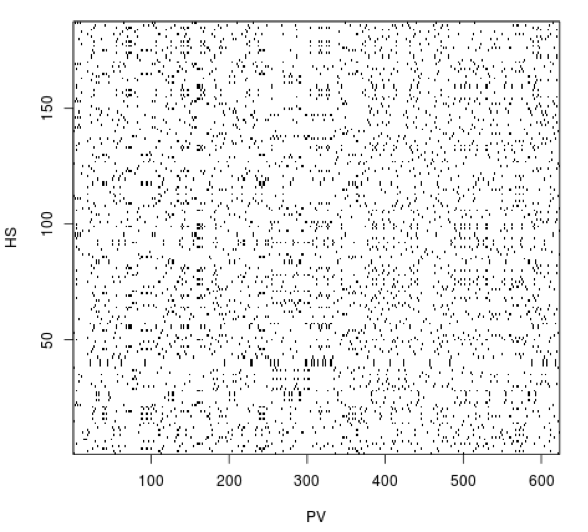
\includegraphics[width=1.0\textwidth]{hs-pv}
   \end{subfigure}
   %\hfill
    \begin{subfigure}[b]{0.35\textwidth}
    \centering
    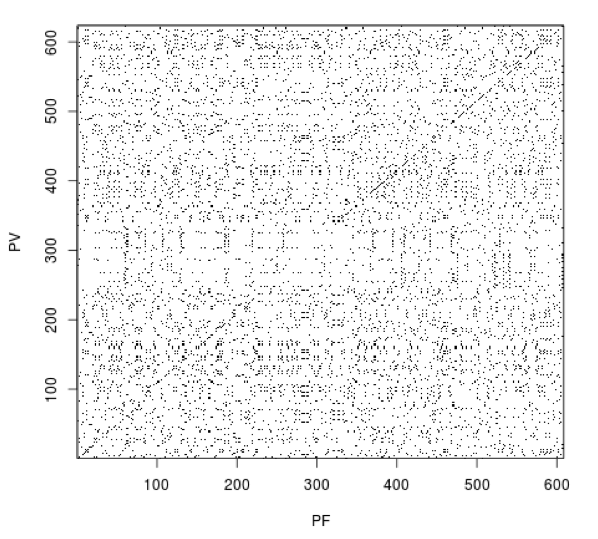
\includegraphics[width=1.0\textwidth]{pv-pf}
   \end{subfigure}
\end{figure}

\end{frame}

\begin{frame}
\frametitle{Comparison via Sequence Alignment 1/2} 
\begin{itemize}%[<+->]
 \item \textbf{Global Sequence Alignment:} an alignment of the full length of two sequences\\
    \textit{we compute Needleman-Wunsch global alignment}
 \item \textbf{Local Sequence Alignment:} an alignment of part of one sequence to part of another sequence\\
   \textit{we compute Smith-Waterman local alignment}
 
%What we transfer is the difference in activity between human and parasites. In more detail, we transfer the difference in activity between a human (where drug is inactive) and one parasite (where drug is active) to another parasite (about which we have little data)
 \end{itemize}
\end{frame}

\begin{frame}
\frametitle{Comparison via Sequence Alignment 2/2} 
%\begin{itemize}%[<+->]

\begin{figure}[h!]
  %\caption{A picture of a gull.}
  \centering
    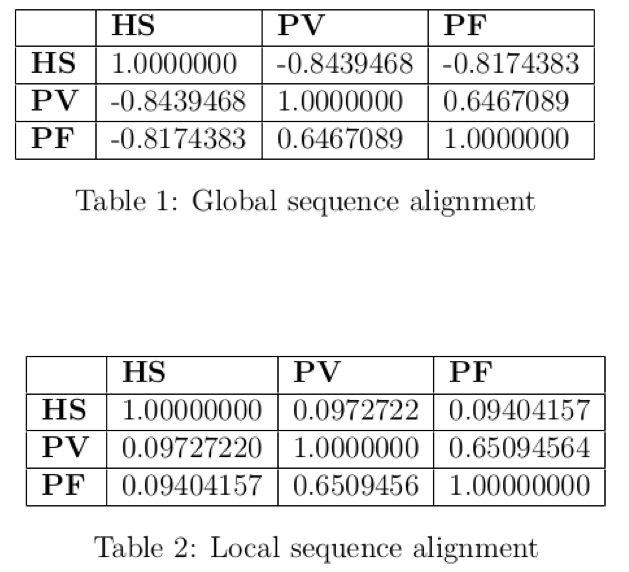
\includegraphics[width=0.7\textwidth]{seq}
\end{figure}

 %What we transfer is the difference in activity between human and parasites. In more detail, we transfer the difference in activity between a human (where drug is inactive) and one parasite (where drug is active) to another parasite (about which we have little data)
 %\end{itemize}
\end{frame}

\end{document}
